\documentclass[11pt, a4paper]{report}
\usepackage[utf8]{inputenc}
\usepackage{float}
\usepackage{array}
\usepackage{amsmath}
\usepackage{amssymb}
\usepackage{amsfonts}
\usepackage{latexsym}
\usepackage{graphicx}
\usepackage{tabularx}
\usepackage{ltxtable}
\usepackage{longtable}
\usepackage{color, colortbl}
\usepackage{caption}
\usepackage{ifpdf}
\usepackage[hidelinks]{hyperref}
\usepackage{url}
\usepackage{xtab}
\usepackage[hmargin=3cm,vmargin=3cm]{geometry}
\usepackage[norsk, english]{babel} 
\usepackage[parfill]{parskip}
\usepackage{pdfpages}
\usepackage{listings}
\usepackage{subfigure}


% Begin chapter numbering
\usepackage[T1]{fontenc}
\usepackage{titlesec, blindtext, color}

\definecolor{gray75}{gray}{0.75}
\newcommand{\hsp}{\hspace{20pt}}
\titleformat{\chapter}[hang]{\Huge\bfseries}{\thechapter\hsp\textcolor{gray75}{|}\hsp}{0pt}{\Huge\bfseries}
% End chapter numbering

% Add numbering to subsubsection
\setcounter{secnumdepth}{3}
\setcounter{tocdepth}{3}

%\newcommand{\newCommandName}{text to insert} % Defines a variable in LaTeX
\newcommand{\comment}[1]{} \comment{This is a block comment wrapped in curly brackets}
%\renewcommand{\thefootnote}{\roman{footnote}}

\definecolor{Gray}{gray}{0.9}

%Header packages
\usepackage{fancyhdr}
\pagestyle{fancy}
\rhead{Chapter: \thechapter}

\begin{document}
\pagenumbering{gobble}

%\begin{titlepage}
\begin{center}
\vspace*{1in}
{\LARGE IT2901 - Informatikk prosjektarbeid II}
\par
\vspace{1cm}


\begin{figure}[ht!]
\centering

\includegraphics[width=25mm]{images/ic_launcher.png}
%\caption{A simple caption}
\label{overflow}
\end{figure}


{\LARGE $\mu$C Software Store}
\par
\vspace{0.6in}
{\LARGE Project Report}
\par
\vspace{0.2in}
{\Large 09\_Arduino}
\par
\vfill
\par
\vspace{0.5in}
Jeppe Eriksen, Bjørn Arve Fossum, Ståle Semb Hauknes,\\ Wilhelm Walberg Schive, Nina Margrethe Smørsgård, Robin Tordly\\
\par
\vspace{0.4cm}
\today %Month Year -formatting?
\end{center}
\end{titlepage}

\newpage

%\begin{abstract}

In cooperation with IDI at NTNU, SINTEF was the contracting customer for this project, hiring the group consisting of six students on the course IT2901.\\
\\
The project's aim was to expand the usability of existing Arduino devices, and simplifying the process of installing new functionality.
This report is an overview of the project of developing the system to do so, and how the work of the developer team evolved alongside the demands and needs of the customer.
The base idea was to create an easy-operable system running on Android based devices for installing compatible applications to the customers' existing Arduino device.
This was done by implementing the STK-500v1 protocol for AVR061 onto the Arduino Uno board, and creating a market-application for Android that handles connection via Bluetooth and data transfer over that protocol, as well as containing the market for browsing of available apps.\\
\\
The development of both the protocol and the app was done in Java, as both was designed to run on Android devices. This was a small challenge as the protocol originally was written in C for the AVR061. Loading of addresses while writing to the Arduino proved to be the thing delaying integrating development of the app and the protocol into one package, requiring modification of requirements.\\
\\
The Arduino side of the software was written in C, but much could be reused from a prior project.

\end{abstract}


\tableofcontents
\newpage
\pagenumbering{arabic}

\chapter{Introduction}
This is the user manual for the $\mu$C Software Store application. It contains all the information needed regarding common use and options. $\mu$C Software Store is an application for the Android platform made as an app store for applications for Arduino based projects. You can browse different applications for Arduino projects and install them through a Bluetooth connection. It is assumed that $\mu$C Software Store, and optionally a QR-code reader, is installed on an Android device and that a properly configured Arduino project with Bluetooth is nearby.\\
\newline
Throughout this document, the application refers to $\mu$C Software Store while an app is one of the applications available within the store.

\chapter{Welcome Screen}
The first screen that will show when entering the application for the first time is the welcome screen. This screen allows the choice between either going directly to the shop or checking devices located in the area. \\
\newline
\begin{figure}[H]
	\centering
	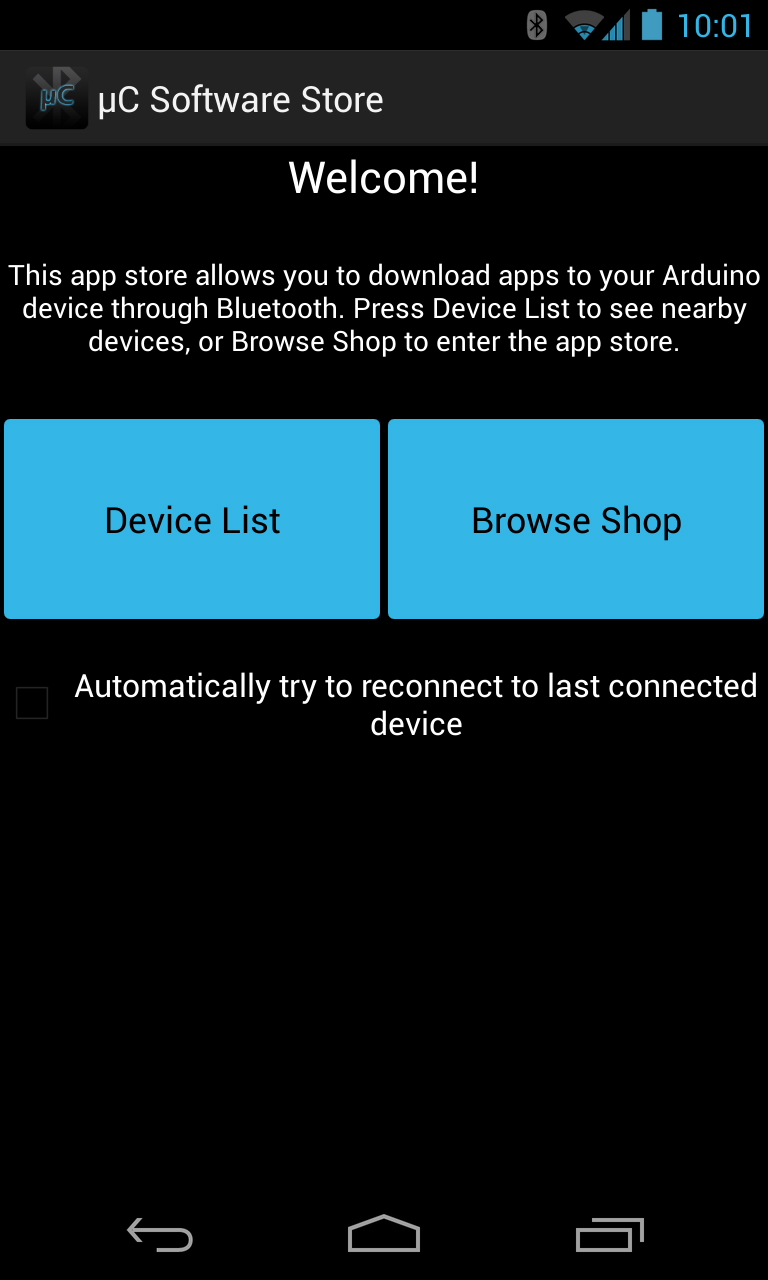
\includegraphics[scale = 0.3]{images/Screenshots/welcome_screen.png}
	\caption{The welcome screen of the application}
\end{figure}

After the first time the application was launched, on the foreground of this screen the application will attempt to automatically reconnect to the last device which was connected through the application. This is an option which can be turned off in the settings. 

\chapter{Device List}
Upon selecting the Device List button from the welcome screen or from the action overflow, this screen will appear. On this screen, Bluetooth devices within the reach of the telephone will appear in a list. If the device you want to connect to doesn't show, or you do not want to connect to a device just yet, you can press either the add device or browse shop button respectively.\\
%Bilde!
\newline
\begin{figure}[H]
	\centering
	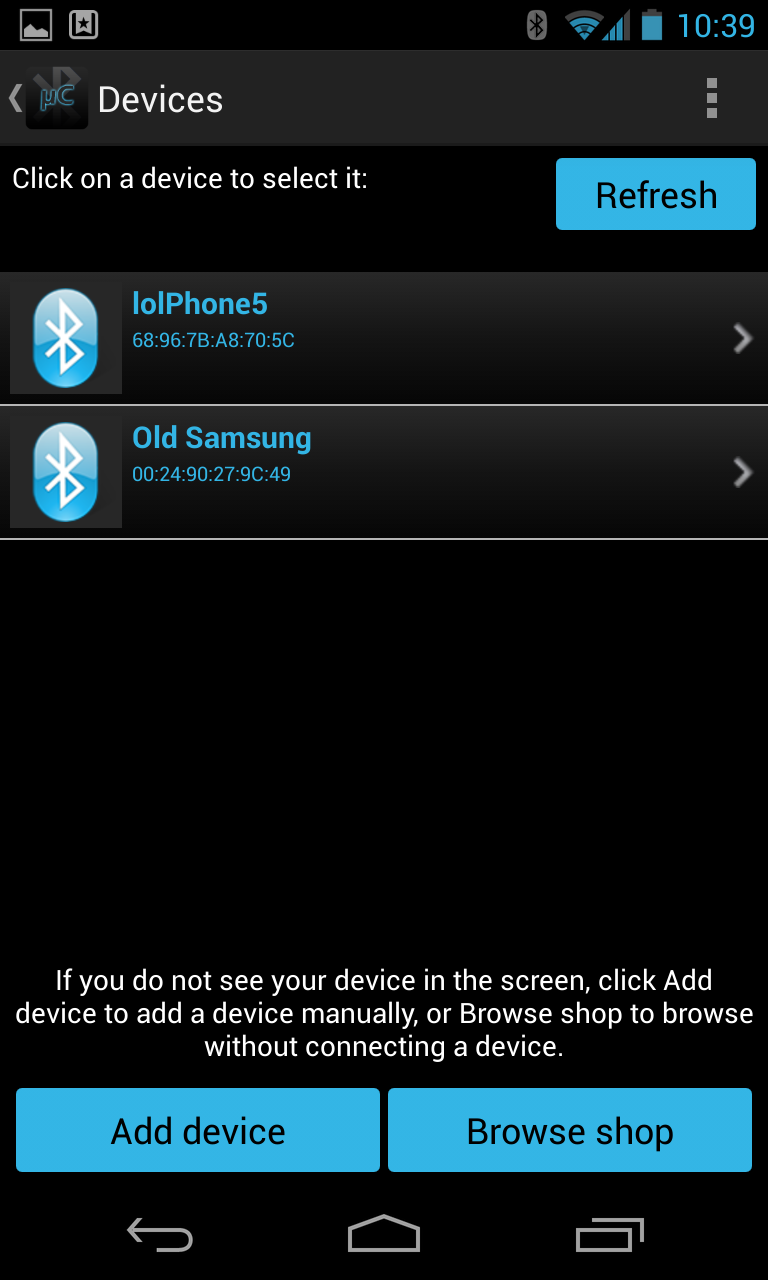
\includegraphics[scale = 0.3]{images/Screenshots/device_list.png}
	\caption{The device list with Bluetooth devices}
\end{figure}
 To connect to a device, simply press the appropriate device in the list and a connection will be established. Some devices require a password in order for connection to be made, you will be prompted on this upon selecting this device. A dialog box will show whether the connection was established and the background of the now connected device in the list will go green to indicate that it is connected. \\
\newline
%nytt bilde med connected
\newline
\begin{figure}[H]
	\centering
	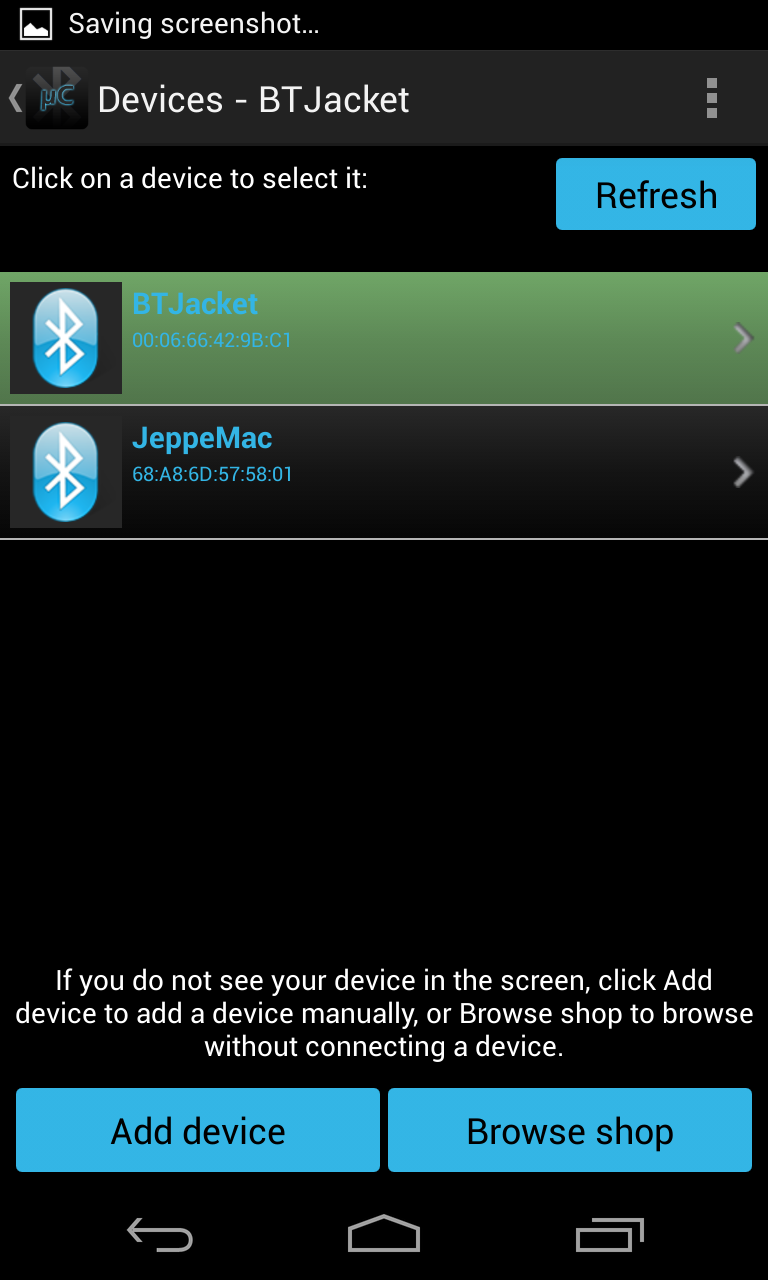
\includegraphics[scale = 0.3]{images/Screenshots/connected.png}
	\caption{The device list when connected to a device}
\end{figure}

\subsection{Adding Device}
Pressing the add device button will give you a choice of how you want to add or connect to a device. You can attempt to connect to a device using either a QR-Code or a serial.
%bilde
\newline
\begin{figure}[H]
	\centering
	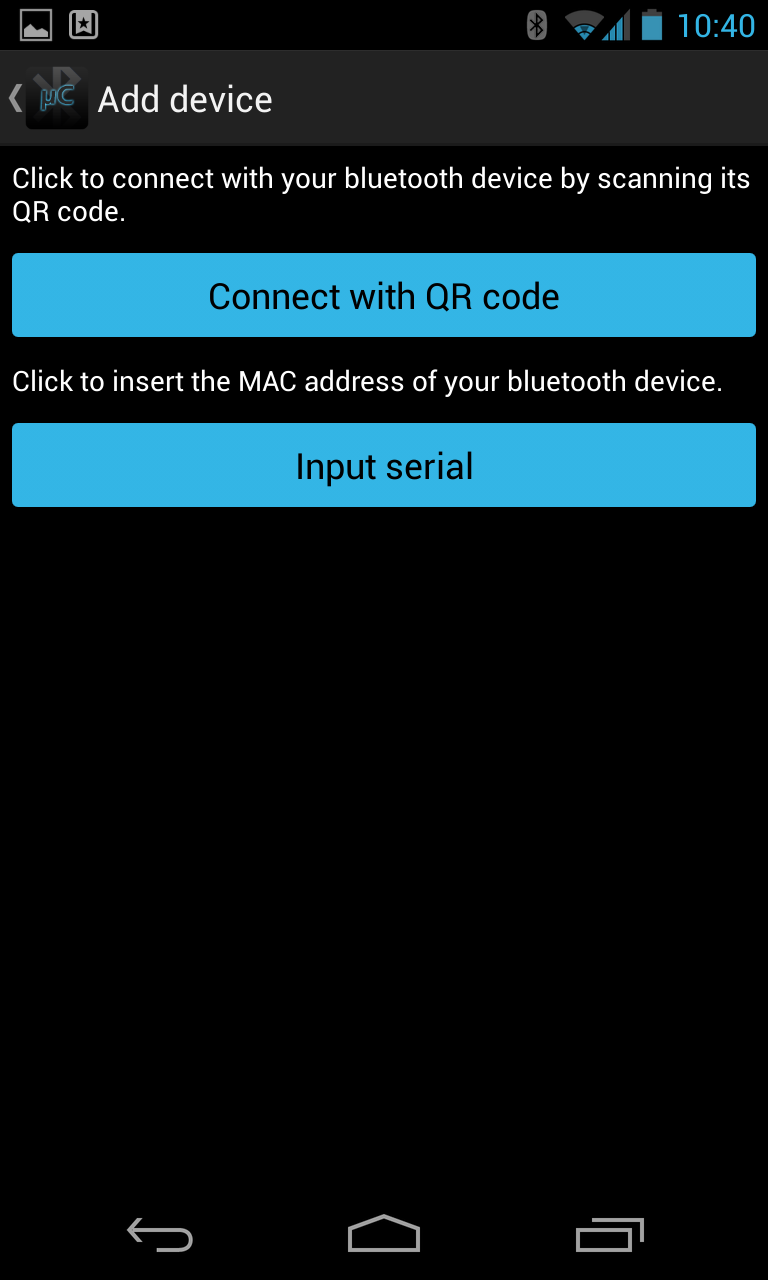
\includegraphics[scale = 0.3]{images/Screenshots/add_device.png}
	\caption{The options for adding devices}
\end{figure}

\subsubsection{QR-Code}
In order for you to connect with a QR-code, an app called BarCodeScanner must first be installed on the Android device. This will allow you to scan a QR-Code which the will enter the MAC address for the device it was made, and a connection will be created.\\

\subsubsection{Serial}
A connection can also be created by typing in a serial, which is the MAC address of the Arduino device. This serial is six groups of hexadecimal digits, meaning 0-9 and a-f, each group separated by a colon (:). You have to include the colon when typing this address, but it is not case sensitive which means you do not have to worry about capital letters.\\

\chapter{The Shop}
The first choice in the shop is the category screen.\\
%bilde av category view
\newline
\begin{figure}[H]
	\centering
	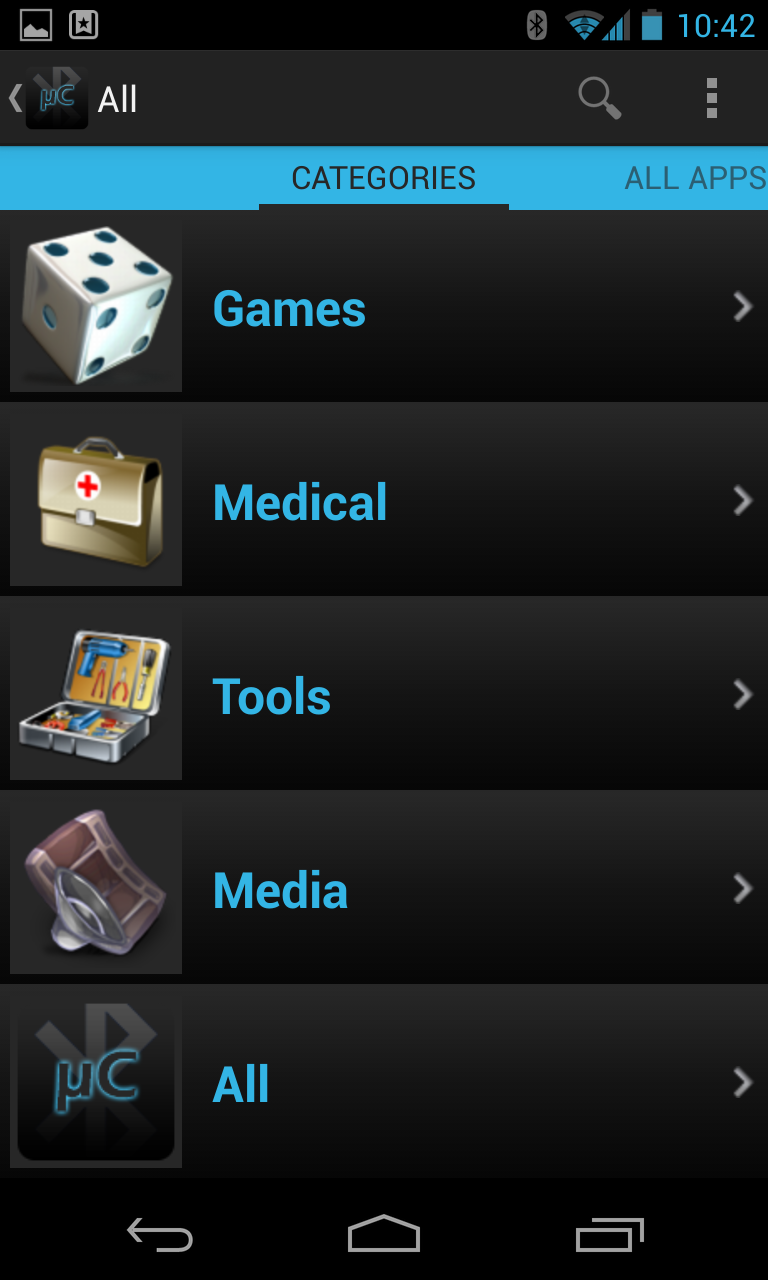
\includegraphics[scale = 0.3]{images/Screenshots/category_view.png}
	\caption{The categories of the shop}
\end{figure}
You can filter through all of the apps in the store through these buttons. You can also browse all the apps together by pressing ``All". There are two ways to sort the apps within the chosen category. Either not at all, which is the first screen that shows after selecting a category, or by the given rating. \\
%bilde av all apps view
\newline
\begin{figure}[H]
	\centering
	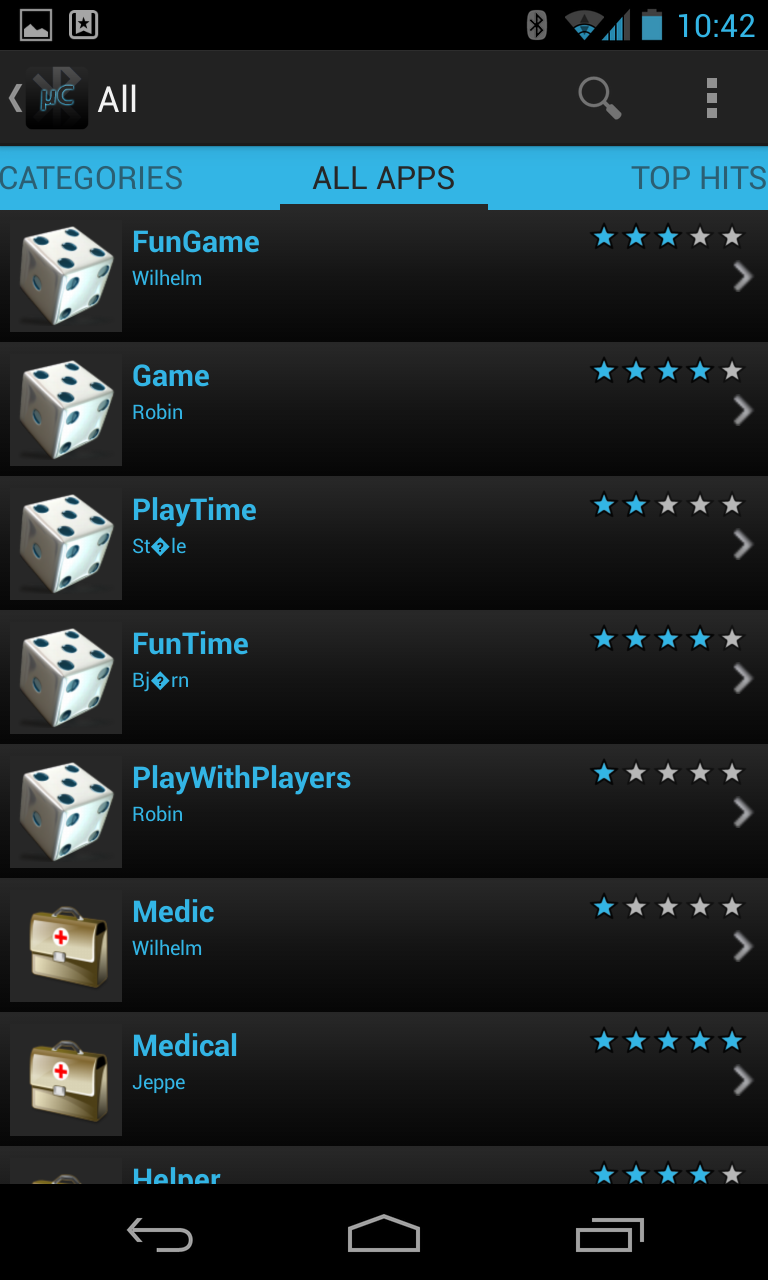
\includegraphics[scale = 0.3]{images/Screenshots/all_apps.png}
	\caption{Screenshot from the shop with all apps shown}
\end{figure}

Each app within the category selected is now shown on the screen. The rating for each app, name of the app, name of the publisher, and the icon of the app is shown for all the apps. The user can go back to the categories by pressing the back button. \\

\subsection{Searching}
Wherever you are in the shop, you can start a search for an app you want. It doesn't matter how old or what buttons you have on your Android device, it is possible to start a search from all buttons and devices. The search results will show after pressing the search button, and if there are no results you will be back at the shop screen with a toast telling you there were no results.

\chapter{App View}
Upon selecting an app in the shop, you will be taken to the app view. This view displays more information about the app you selected, like required hardware, pictures, developer and most importantly, an install button. 
%bilde
\newline
\begin{figure}[H]
	\centering
	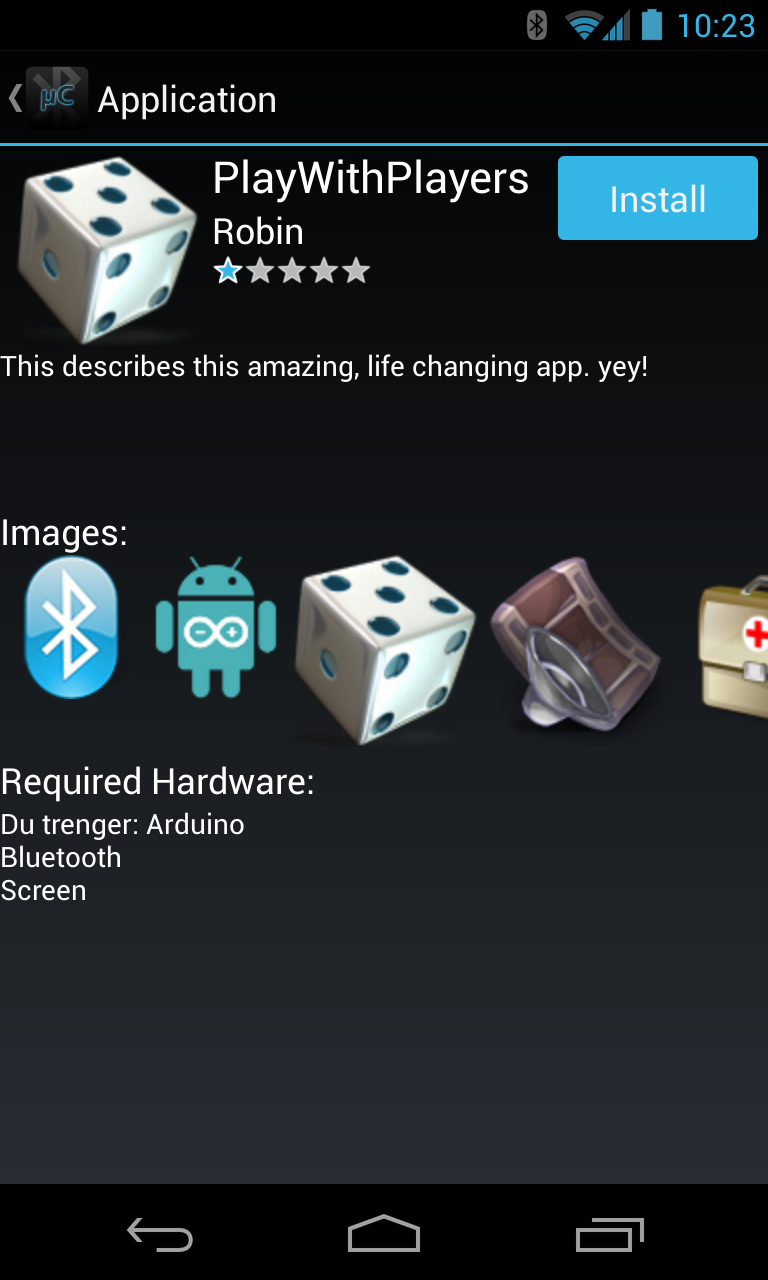
\includegraphics[scale = 0.3]{images/Screenshots/app_view.png}
	\caption{App View showing information about a single app}
\end{figure}
Upon pressing the install button, as long as you are connected to an Arduino device you will be first asked to confirm the action. If you do the install will begin. If, however, you are not connected to a device, a dialog will open with the options of either going back to the app view, or go directly do the device list to connect to a device.

\chapter{Settings}
The settings available in $\mu$C Software Store are as follows:

\begin{description}
	\item[Hide/Show incompatible] \hfill \\
		Allows you to hide/show all apps not compatible with the currently connected device.
	\item[Connected device] \hfill \\
		Shows the currently connected or the last connected device. 
	\item[Automatically reconnect] \hfill \\
		 Controls whether the application should attempt to automatically reconnect at the welcome screen when reentering the application.
	\item{Hide other devices}\hfill \\
		Allows the option of hiding/showing devices in the device list which does not properly identifies themselves as an Arduino device. 
\end{description}


\newpage
\addcontentsline{toc}{chapter}{List of Tables}
\listoftables
\addcontentsline{toc}{chapter}{List of Figures}
\listoffigures
\addcontentsline{toc}{chapter}{Bibliography}
\bibliographystyle{plain}
%% We use MLA standard for citation. Create your citations at:
% \url{http://citationmachine.net/index2.php?reqstyleid=0&stylebox=1

% Remember to update the bibliography number as you add or remove bibitems.
\thispagestyle{plain}

\begin{thebibliography}{21}

	\bibitem{baudrate}{
		\emph{electronicdesign.com}
		N.P.. Web. 01 May 2013
		<\url{http://electronicdesign.com/communications/what-s-difference-between-bit-rate-and-baud-rate}>
	}

	\bibitem{kruchten}{
        Kroll, P., and P. Kruchten. \emph{The rational unified process made easy: A practitioner's guide to the rup}. Boston, MA: Addison-Wesley Professional, 2003. eBook.
    }

	\bibitem{scrum}{
		\emph{Scrum.org}.
		N.p.. Web. 13 Mar 2013
		<\url{http://www.scrum.org/Resources/What-is-Scrum}>.
		}

	\bibitem{sommerville}{
		Sommerville, Ian. \emph{Software Engineering}. 9th ed. Boston: Pearson Custom Publishing, 2011. Print.
	  	}

    \bibitem{poppendieck}{
        Poppendieck, M., and T. Poppendieck. \emph{Lean software development, an agile toolkit}. Addison-Wesley Professional, 2003. Print.
        }

    \bibitem{rn-42}{"Bluetooth Module - RN-42." Sparkfun.com. Sparkfun. Web. <https://www.sparkfun.com/products/10393>. 
    }

	\bibitem{hc-05}{"Bluetooth Module - HC-05." Iteadstudio.com. Itead Studio. Web. <ftp://imall.iteadstudio.com/Modules/IM120723009/DS_IM120723009.pdf>. 
    }

	\bibitem{testing-overview}{
		\emph{Microsoft.com}.
		N.p.. Web. 13 Mar 2013
		<\url{http://msdn.microsoft.com/en-us/library/aa292191(v=vs.71).aspx}>
	}

		\bibitem{unit-testing1}{
		\emph{Microsoft.com}.
		N.p.. Web. 13 Mar 2013
		<\url{http://msdn.microsoft.com/en-us/library/aa292197(v=vs.71).aspx}>
	}
	
	\bibitem{unit-testing2}{
		\emph{GeoSoft.no}.
		N.p.. Web. 13 Mar 2013
		<\url{http://geosoft.no/development/unittesting.html}>
	}

	\bibitem{unit-testing3}{
		\emph{Android.com}.
		N.p.. Web. 13 Mar 2013
		<\url{http://developer.android.com/tools/testing/testing\_android.html}>
	}

	\bibitem{Nielsen}{
		Nielsen, Jakob. ``Why you only need to test with 5 users.'' \emph{NNgroup.com}. N.p., 19 Mar 2000. Web. 16 Apr 2013. <\url{http://www.nngroup.com/articles/why-you-only-need-to-test-with-5-users/}>.
	}


    \bibitem{AVR068}{
        \emph{Atmel.com}.
        N.P.. Web. 8 Feb 2013
        <\url{http://www.atmel.com/Images/doc2591.pdf}>
    }
    
    \bibitem{StkBoot}{
		\emph{Google.com}
		N.P.. Web. 25 Mar 2013
		<\url{https://code.google.com/p/stkboot/}>
	}
	
	\bibitem{uOS-Embedded}{
		\emph{Google.com}
		N.P.. Web. 25 Mar 2013
		<\url{https://code.google.com/p/uos-embedded/}>
	}

    \bibitem{AVR061}{
        \emph{Atmel.com}.
        N.p.. Web. 26 Mar 2013
        <\url{http://www.atmel.com/Images/doc2525.pdf}>
    }
    	
	\bibitem{validation-testing}{
		\emph{Buzzle.com}.
		N.p.. Web. 13 Mar 2013
		<\url{http://www.buzzle.com/articles/validation-testing.html}>
	}
    	
    \bibitem{integration-testing2}{
		\emph{Microsoft.com}.
		N.p.. Web. 13 Mar 2013
		<\url{http://msdn.microsoft.com/en-us/library/aa292128(v=vs.71).aspx}>
	}
	
	\bibitem{functional-testing}{
		\emph{Wikipedia.org}.
		N.p.. Web. 13 Mar 2013
		<\url{http://en.wikipedia.org/wiki/Functional\_testing}>
	}

    \bibitem{android-dev-guide}{
    	\emph{Android.com}
    	N.p.. Web. 5 May 2013
    	<\url{http://developer.android.com/design}>
    }

    \bibitem{git-branch}{
    	\emph{http://git-scm.com/}
    	N.p.. Web. 12 May 2013
    	<\url{http://git-scm.com/book/en/Git-Branching-What-a-Branch-Is}>
    }

    \bibitem{websequencediagrams}{
    	\emph{http://www.websequencediagrams.com/}
    	N.p.. Web 12 May 2013
    	<\url{http://www.websequencediagrams.com/}>
    }
    
    \section*{Source of images}
    This section containts the all the sources for all the images used in the report. The images and sources that are not listed here is made by the project team. \\

    Figure~\ref{fig:sintef} in section~\ref{sec:sintef} : \\
    N.P.. Web. 19 Apr 2013\\
	<\url{http://www.sintef.no}> \\

	Figure~\ref{fig:ntnu} in section~\ref{sec:ntnu} : \\
	N.P.. Web. 19 Apr 2013\\
	<\url{http://www.ntnu.no}> \\

	Figure~\ref{fig:googleplay} in section~\ref{sec:googleplay} \\
	N.P.. Web. 13 Mar 2013\\
	<\url{http://droidtrends.com/wp-content/uploads/2012/07/Google-Play-Store-APK-3.7.15.jpg}> \\

	Figure~\ref{fig:pebblewatch} in section~\ref{sec:pebblewatch} : \\
	N.P.. Web. 19 Apr 2013\\
	<\url{http://getpebble.com/}> \\

	Figure~\ref{fig:SimpleArduinoWiring} in section~\ref{sec:SimpleArduinoWiring} : \\
	N.P.. Web. 19 Apr 2013\\
	<\url{http://fritzing.org/}> \\

	Figure~\ref{fig:rup} in section~\ref{sec:rup} \\
	N.P.. Web. 19 Apr 2013\\
	<\url{http://www.c3ns.com/c3nsservices_3.html}> \\
	
\end{thebibliography}


\newpage
\addcontentsline{toc}{chapter}{Appendixes} %this line may break your compilation, and may require recompiation
\appendix
%\chapter{Project documents}
\label{appendix-project-documents}
Here documents produced in relation to the project will be presented. Both status reports and activity plans were to be created and delivered to the supervisor every other week. 

\section{Status report example}
%Tried to make it look as much as the actual status report as possible. That's why it looks a bit funny.
Below is a copy of an status report made by the group for the supervisor. This status report is for the weeks 6 and 7.\\
\newline

\textbf{1. Introduction}\\
These two weeks were the first weeks of project work, since little could be done prior to meeting the customer. During the first week there was one member missing.\\
\newline

\textbf{2. Progress summary}\\
In this two-week period we have completed on average 68\% of the work scheduled on the activity plan. We believe that we still are on schedule according to the milestones set by the customer. The work that was done was in general related to the design of the final product and making sure we have all the required libraries, licenses and other factors that need to be in order before we start programming the actual product.\\
\newline

\textbf{3. Open / closed problems}\\
\newline
\textbf{Open:}
\begin{itemize}
	\item{New requirements: friendlier bluetooth device pairing}
	\item{Bluetooth connection: need a bluetooth module to the arduino}
	\item{Not documented preexisting code}
	\item{Decide on a product name}
\end{itemize}
\vspace{8mm}

\textbf{Closed:}
\begin{itemize}
	\item{Lacking source code: Will not use the compiled program in question}
	\item{Licenses: separate out licensed components into separate projects}
\end{itemize}
\vspace{8mm}

\textbf{4. Planned work for next period}\\
For next period we will have to complete the designs of the project and complete version 0.1 to show to the customer.\\
\newline

\textbf{5. Updated risks analysis}\\
\begin{itemize}
	\item{License incompatibility: impact has gone down from 8 to 7. Importance has gone down from 10 to 8. This is because of information from the customer about ways to circumvent this issue (as mentioned above).}
\end{itemize}

\section{Activity plan example}
Below is an example of an activity plan made by the group for the supervisor. This activity plan is for the weeks 6 and 7.\\

\begin{figure}[H]
\makebox[\textwidth][c]{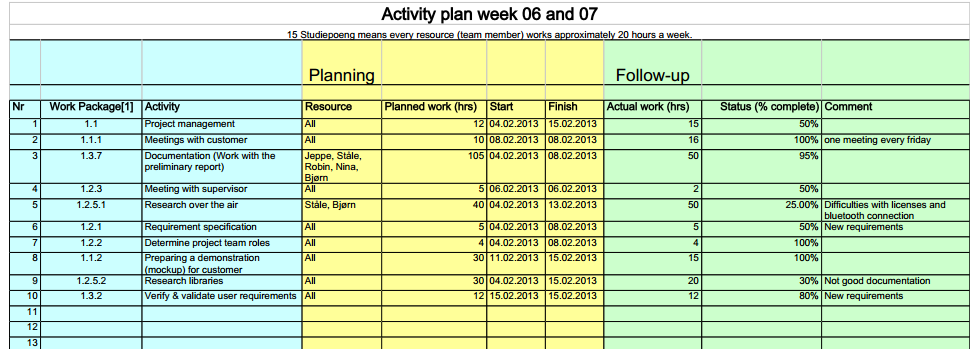
\includegraphics[width=1.3\textwidth]{images/activity_plan_example.png}}
\caption{Example of activity plan for the weeks 6 and 7}
\end{figure}

%\chapter{Iterations}

This section contains an overview and a summary of each iteration of this project. The project was split into
iterations of two weeks, and the content is based on the activity plan and the status report that was delivered to the supervisor. In each iteration the use cases described in chapter ~\ref{usecases} is shown to present what the group was working on.

\section{Iteration 1}
Week 6 and 7
\subsection{Summary}
	These were the first two weeks of the project and the first group meeting was arranged.	Meeting with the customer to get the requirement specification and understanding of the projects goal was done.	Required libraries, licenses and other factors was taken in account before the group could start developing. No use cases were generated in this iteration, as basic research and planning had to be done before scenarios could be generated.
\subsection{Overview}
\begin{itemize}
	\item{Confirm understanding of the task}
	\item{Ideas for identifying the capabilities of an Arduino device and how to communicate these to the store client}
	\item{Investigate potential solutions to facilitate over the air installation of Arduino applications}
	\item{Start design the GUI for the Android application}
	\item{Research on Apache licenses}
	\item{Meeting with customer}
\end{itemize}

\section{Iteration 2}
Week 8 and 9
\subsection{Summary}
	Architectural work and design of the user interface of the Android application. Positive feedback on the GUI was received from the customer. Design of use cases and further research was performed.
\subsection{Overview}
\begin{itemize}
	\item{Think architectural}
	\item{Designing of GUI}
	\item{Research on over the air implementation}
	\item{Research Ubicollab libraries}
	\item{Use iJacket - generic application, Bluetooth connection code}
	\item{Implement a first sketch of the content provider}
	\item{Meeting with customer}
\end{itemize}

\section{Iteration 3}
Week 10 and 11
\subsection{Summary}
	Focus on Bluetooth connection and over the air implementation was prioritized these weeks. The application was taking form and the bugs were beginning to show up. Use cases 2, 3, 4 and 5 were in focus during this iteration. There were some issues with over the air because of incompatible licenses and much work was put into research. The Android application was estimated to be 50\% complete.

\subsection{Overview}
\begin{itemize}
	\item{Research Ubicollab libraries}
	\item{Finish design of the GUI}
	\item{Establish a Bluetooth connection between Android and Arduino}
	\item{Implement last draft of the content provider}
	\item{Meeting with customer}
\end{itemize}

\section{Iteration 4}\label{Iteration4}
Week 12 and 13
\subsection{Summary}
	This iteration became critical when it was discovered that existing implementations of the STK500 protocol were either incompatible with the required Apache v.2 license or not compatible with Android. An emergency meeting with the customer took place and it was decided to implement the STK500 protocol in Java. Developing the Sync Adapter was removed from the requirements, and the focus was moved to implementing the protocol as a library. Use cases 2, 3 and 4 were in focus during this iteration.

\subsection{Overview}
\begin{itemize}
	\item{Emergency meeting with customer}
	\begin{itemize}
		\item{Not possible to use existing solutions of STK500 protocol}
		\item{Agreement on implementing the STK500 in Java ourselves as a library}
	\end{itemize}
	\item{Research on STK500}
	\item{Unit test sketches}
	\item{Continued work on develop the Android application}
\end{itemize}

\section{Iteration 5}
Week 14 and 15
\subsection{Summary}
	Good progress and much was done. The group was more optimistic about the implementation of the protocol and the development of the application was almost complete.	The group was now split into two, where one group was writing the protocol, and the other group was writing Unit tests and polishing the last parts of the application. Use cases 4, 5 and 7 were in focus during this iteration.

\subsection{Overview}
\begin{itemize}
	\item{Added storage of hex-files to content provider}
	\item{Writing Robotium unit tests}
	\item{Writing the STK500 protocol in Java/Android}
	\item{Finishing the Android application except for the STK500 part}
	\item{Meeting with customer}
\end{itemize}

\section{Iteration 6}
Week 16 and 17

\subsection{Summary}
	Unexpected issues with programming the Arduino nearly caused the implementation to fail, requiring a meeting with the customer.
Suggestions for alternate solutions were presented, and it was decided to work in parallel on some of them. The customer was to attempt to ask some experts in the field for some code review.
Shortly after the meeting the problem was resolved.

\subsection{Overview}
\begin{itemize}
    \item{Meeting on protocol implementation problems}
    \item{Problem resolution}
	\item{Implement the STK500 to the Android application}
\end{itemize]

\section{Iteration 7}
Week 18 and 19

\subsection{Summary}
These were the last two weeks scheduled for the project. 

The final parts of the application were completed and the STK500 was implemented into the application as a library.
	A workshop with the customer at SINTEF was held, and an acceptance test and a usability test were performed. Most of the time was spent on completing the documentation.

\subsection{Overview}
\begin{itemize}
	\item{Workshop for SINTEF}
		\begin{itemize}
			\item{Demonstrate our finish application}
			\item{Acceptance testing}
			\item{Usability testing}
		\end{itemize}
\end{itemize}


\end{document}
